\documentclass{article}

\usepackage[french]{babel}
\usepackage[utf8]{inputenc}
\usepackage[T1]{fontenc}
\usepackage{amsmath}
\usepackage{amssymb}
\usepackage{amsthm}
\usepackage{comment}
\usepackage{dsfont}
\usepackage{fullpage}
\usepackage{glossaries}
\usepackage{graphicx}
\usepackage{hyperref}
\usepackage{xspace}
\usepackage[
    style=numeric,
    sorting=none
]{biblatex}

\newglossaryentry{blockchain}
{
    name=blockchain,
    description={une base de données distribuée 
    constituée d’une chaîne de blocs liés et sécurisés 
    par des hachés cryptographiques.}
}

\newacronym{aes}{AES}{Advanced Encryption Standard}
\newacronym{dns}{DNS}{Domain name system}
\newacronym{ecdlp}{ECDLP}{Elliptic curves discrete logarithm problem}
\newacronym{esp}{ESP}{Encapsulation security payload}
\newacronym{ip}{IP}{Internet Protocol}
\newacronym{ipsec}{IPSec}{Internet Protocol Security}
\newacronym{p2p}{P2P}{Pair à pair}
\newacronym{p2pkh}{P2PKH}{Pay-to-Public-Key-Hash}
\newacronym{ssl}{SSL}{Secure Sockets Layer}
\newacronym{ringct}{Ring CT}{Ring Confidential Transactions}
\newacronym{tcp}{TCP}{Transmission Control Protocol}
\newacronym{tor}{Tor}{The Onion Router}
\newacronym{tga}{TGA}{Transaction graph analysis}
\newacronym{utxo}{UTXO}{Somme des sorties non dépensées (\og \textit{unspent transactions outputs}\fg)}
\newacronym{vpn}{VPN}{Virtual Private Network}

\makeglossaries

\title{Anonymat dans les blockchains}
\author{Louis de Campou}
\date{14/09/2023}

\bibliography{sources.bib}

\newtheorem{definition}{Définition}
\newtheorem{example}{Exemple}
\newtheorem{proposition}{Proposition}

\begin{document}

\maketitle

\newpage
\tableofcontents

\newpage
\section{Introduction}
\noindent
Les échanges financiers sur Internet reposent presque exclusivement via les institutions 
financières, qui agissent comme tiers de confiance pour le traitement des paiements 
électroniques.\\
L'anonymat et la décentralisation sont des caractéristiques intéressantes à explorer
pour le futur des paiements électroniques, à cause des inévitables conflits d'intérêt 
entre les autorités centrales et les utilisateurs.\\
En 2008, \og Bitcoin\cite{bitcoin_wp}: A Peer-to-Peer Electronic Cash System \fg publié 
sous le pseudonyme Satoshi Nakamoto, a partagé une solution permettant à deux parties 
d'échanger de la monnaie électronique.\\
La particularité de cette solution est la suppression de ce modèle de confiance 
par l'ajout d'une preuve cryptographique.

\bigskip

%Bitcoin a été la première solution pair à pair, pseudonyme et voulue décentralisée.\\
À ses débuts, Bitcoin a été qualifié comme une monnaie électronique \og anonyme \fg
et non pseudonyme.
Le pseudonymat de l'utilisateur repose sur l'hypothèse que son pseudonyme, 
l'adresse d'un compte dérivée à partir d'une paire de clefs, ne soit pas lié à sa 
véritable identité.
D'autres vulnérabilités peuvent être exploitées par un adversaire souhaitant désanonymiser 
des utilisateurs. Le réseau Bitcoin est un réseau \acrshort{p2p} où les participants 
sont interconnectés via un canal \acrshort{tcp} non chiffré. Les participants du réseau, plus connus 
sous le nom de noeuds, maintiennent à jour une liste d'adresses \acrshort{ip} de leurs noeuds voisins. 
Après qu'une transaction ait été créée, celle-ci est propagée aux noeuds voisins du noeud 
originaire de la transaction, qui vont eux-mêmes propager la transaction à leurs propres 
noeuds voisins. Si un noeud contrôlé par un adversaire peut s'assurer qu'une connexion entrante 
faisant part d'une transaction provient de l'auteur même de la transaction, l'adversaire peut
corréler l'adresse \acrshort{ip} du noeud et la transaction, compromettant l'anonymat.
Une atténuation est d'utiliser un \acrshort{vpn} (de confiance !) ou \acrshort{tor} afin d'offusquer sa 
réelle adresse \acrshort{ip}.
Un autre risque provient de la nature publique des transactions (voir 2.2) et de
l'exploitation du \acrshort{tga}.

\bigskip

Depuis, des protocoles comme CryptoNote\cite{monero_wp} à l'origine de Monero, ont émergé 
mettant l'accent sur la vie privée et l'anonymat. Le \acrshort{tga} n'est plus exploitable car : 
\begin{itemize}
    \item les entrées de transaction ne sont plus liées à un seul émetteur grâce 
    aux signatures en anneau 
    \item une adresse de réception unique est générée par l'émetteur pour chaque transaction grâce
    aux adresses jetables (\og one-time addresses \fg)
    \item les montants sont rendus confidentiels grâce à \acrshort{ringct}
    %RingCT est utilisé pour cacher le montant de la transaction en combinant plusieurs 
    %transactions avec le même montant de sortie en une seule transaction.
\end{itemize}

\medskip 
\noindent
Le prochain chapitre sera consacré à introduire la notion d'espaces de noms (\og \textit{namespace} \fg).
L'un des objectifs de ce travail est d'énumérer les espaces de noms en rapport à l'anonymat 
ainsi que des relations entre espaces de noms pouvant compromettre l'anonymat ou au contraire 
le garantir.

\section{Espaces de noms}
\begin{definition}[Espace de noms]
    Un espace de noms est un ensemble fini d'éléments, qui sont des noms.
\end{definition}

\begin{example}
    Une adresse \acrshort{ip}v4 est un espace de noms,
    composée d'une chaîne binaire de 32 bits,
    avec un total de $2^{32}$ valeurs.
\end{example}

\begin{example}
    Une clef publique Bitcoin est un espace de noms, 
    composée d'une chaîne binaire de 256 bits, 
    avec un total de $2^{256} - 2^{32} - 977$ valeurs\cite{bitcoin_secp}.
\end{example}

\begin{proposition}[Composition]
    Un espace de noms peut être une composition de deux ou plusieurs 
    espaces de noms.\\
    Soient 2 espaces de noms A et B, la composition de ces 2 espaces 
    est définie comme un espace de noms C, étant le produit cartésien 
    de A et B : $C = A \times B$
\end{proposition}

\begin{example}
    Soient A une adresse Bitcoin et B une adresse \acrshort{ip}, 
    un portefeuille C hébergé sur une plateforme d'échange peut être représenté 
    tel que : $C = btc\_addr \times ip\_addr$ 
\end{example}

\begin{proposition}[Résolution]
    Un espace de noms peut être résolu en un autre espace de noms.\\
    Soient 2 espaces de noms A et B, la résolution de A en B se définit telle que 
    $\Gamma : A \longrightarrow B$
\end{proposition}

\begin{example}
    Soient A un nom d'hôte et B une adresse \acrshort{ip}v4, 
    le protocole \acrshort{dns} permet de résoudre une adresse \acrshort{ip}v4 
    à partir d'un nom d'hôte ; 
    $\Gamma : hostname \longrightarrow ip\_addr$
\end{example}



\subsection{Adresse Bitcoin \& Monero}
Dans le contexte d'une \textit{\gls{blockchain}}, une adresse est un espace de noms qui sert 
de mécanisme de routage dans un système distribué. Une adresse 
Bitcoin\cite{bitcoin_address} (\acrshort{p2pkh}) est composée de 160 bits.
Un espace d'adressage fait référence au nombre d'adresses disponibles dans un espace 
donné, il est de $2^{160}$ pour une adresse Bitcoin. 
Chaque adresse, étant la sortie du haché de la clef publique correspondante, peut être 
considérée comme une clé unique.

\bigskip 
\noindent
Les adresses Bitcoin \& Monero\cite{monero_address, monero_address2} sont définies 
ci-dessous respectivement.\\
$G$ représente un point de base de la courbe elliptique (secp256k1\cite{bitcoin_secp} 
pour Bitcoin et Ed25519\cite[5]{monero_wp} pour Monero).

\begin{table}[!ht]
    \centering
    \begin{tabular}{|l|l|l|}
    \hline
        espace & taille en bits & description \\ \hline
        priv key $k$ & 256 & génération de bits pseudo-aléatoire \\ \hline
        pub key $K$ & 256 & $K=kG$ \\ \hline
        address & 160 & base58(0x00 + ripemd160(sha256($K$)) + checksum) \\ \hline
        balance & ~ & \acrshort{utxo} \\ \hline
    \end{tabular}
    \caption{Adresse Bitcoin}
\end{table}

\begin{table}[!ht]
    \centering
    \begin{tabular}{|l|l|l|}
    \hline
        espace & taille en bits & description \\ \hline
        priv spend key $k^s$ & 256 & génération de bits pseudo-aléatoire \\ \hline
        priv view key $k^v$ & 256 & $k^v$ = $H(k^s)$ \\ \hline
        pub spend key $K^s$ & 256 & $K^s = k^sG$ \\ \hline
        pub view key $K^v$ & 256 & $K^v = k^vG$ \\ \hline
        address & 552 & base58(0x12 + $K^s||K^v$ + checksum) \\ \hline
        open alias & ~ & nom d'hôte associé à une adresse \\ \hline
        balance & ~ & \acrshort{utxo} \\ \hline
    \end{tabular}
    \caption{Adresse Monero}
\end{table}

\noindent 
La somme de contrôle d'une adresse Bitcoin est égale à : 
sha256(sha256(0x00 + ripemd160(sha256($K$))))[0:31]\\
La somme de contrôle d'une adresse Monero est égale à : 
keccak256(0x18 + $K$)[0:31]

\bigskip 

\begin{itemize}
    \item Les clefs Monero sont deux fois plus grandes que les clefs Bitcoin
    \item Les adresses Monero possèdent 392 bits de plus que les adresses Bitcoin
    \item Monero scinde les clefs en 2 usages : \og \textit{spend} \fg pour défenser 
    des fonds et \og \textit{view} \fg pour obtenir le solde et l'historique de transactions
    d'une adresse
    \item Le solde et l'historique de transactions d'une adresse Bitcoin sont publiques.
    Contrairement à Monero, où l'on peut choisir de communiquer $k_v$
    \item Dans une transaction Bitcoin, les adresses et les montants associés 
    sont publiques tandis que Monero anonymise ces informations.
\end{itemize}
    
\subsection{Transaction Bitcoin \& Monero}
Une transaction (\og tx \fg) est un objet contenant plusieurs champs dont certains champs sont 
des espaces de noms (adresse) et d'autres sont des métadonnées (horodatage).\\
Une transaction représente un mouvement de monnaie d'une adresse à une autre, 
signée avec la clef privée de l'expéditeur, qui souhaite réattribuer la possession d'une 
certaine quantité de monnaie à une adresse de destination spécifiée dans la transaction.\\
Plus précisément, une transaction consiste en :
\begin{itemize}
    \item un ensemble d'entrées (\acrshort{utxo}). Chaque entrée contient un montant associé
    \item un ensemble de sorties ou d'adresses de destination
    \item un montant à transférer à chaque sortie
\end{itemize}

\medskip
\noindent
Les transactions Bitcoin \& Monero sont définis ci-dessous respectivement.\\

\begin{table}[!ht]
    \centering
    \begin{tabular}{|l|l|l|}
    \hline
        espace & taille en bits & description \\ \hline
        hash & 256 & haché de la transaction \\ \hline
        input & 160 & adresse(s) d'entrée \\ \hline
        output & 160 & adresse(s) de sortie \\ \hline
        value & ~ & montants associés aux adresses d'entrée et de sortie \\ \hline
        signature & ~ & preuve que l'expéditeur a autorisé la transaction \\ \hline
    \end{tabular}
    \caption{Transaction Bitcoin}
\end{table}

\begin{table}[!ht]
    \centering
    \begin{tabular}{|l|l|l|}
    \hline
        espace & taille en bits & description \\ \hline
        hash & 256 & haché de la transaction \\ \hline
        input & 256 & image(s) clé(s) \\ \hline
        output & 256 & adresse(s) jetable(s) \\ \hline
        %extra & ~ & stockage de donnée arbitraire par le mineur \\ \hline
        payment id & 64 & chaîne de caractères unique permettant d'identifier une transaction \\ \hline
        ring signature &  & preuve que l'expéditeur a autorisé la transaction \\ \hline
    \end{tabular}
    \caption{Transaction Monero}
\end{table}

\section{Méthodes d'anonymat}
Soit un ensemble d'agents $(A_1,...,A_n)$ qui s'échangent des messages sur un canal 
de communication par défaut unidirectionnel (et bidirectionnel lorsque précisé). 
Un agent peut être un émetteur ou/et un récepteur. Tout message transite vers un système d'anonymat
dans un modèle de boîte noire.
Selon la nature de la méthode d'anonymat utilisée, un agent peut être dénoté par 
une adresse \acrshort{ip}, une clef publique..
Le canal de communication est surveillé par un observateur, qui souhaite par exemple 
connaître l'identité de l'émetteur ou du récepteur d'un message.
Cet observateur est un adversaire honnête mais curieux\cite[2]{hbc}, un participant légitime qui ne s'écarte pas 
du protocole défini mais tente d'obtenir toutes les informations possibles à partir 
des messages reçus légitimement. Les \textit{\gls{blockchain}s} Bitcoin et Monero étant 
publiques, l'observateur a accès possiblement en lecture à toutes les transactions 
publiées sur ces registres. On s'intéressera principalement à l'anonymat de l'émetteur, 
le principe est analogue pour l'anonymat du récepteur. L'anonymat de l'émetteur 
consiste à être indistinguable\cite{anon_term} au sein d'un ensemble, l'ensemble d'anonymat 
(\og \textit{anonymity set}\fg). Il y a un ensemble d'émetteurs possibles
et l'observateur ne peut pas faire la distinction entre les émetteurs de cet 
ensemble. L'observateur souhaite connaître quel émetteur parmi l'ensemble d'anonymat 
est à l'origine d'un message, il assigne une probabilité pour chaque émetteur. Deux méthodes d'anonymat sont analysées : les adresses jetables et les signatures en anneau.\\
D'autres méthodes auraient pu être explorées :
\begin{itemize}
    \item Mixeur : service qui permet d'offusquer la relation entre entrées et sorties d'une transaction, et préserver l'anonymat relationnel. Ce service peut être centralisé, c'est à dire qu'il dépend d'un serveur central pour effectuer le mixing.
    Un problème de confiance est inhérent avec cette approche : il n'y a aucune certitude que ce type de service ne conserve des logs (adresses \textit{blockchain}, adresses \acrshort{ip}..) ou redistribue les jetons. 
    \item \acrshort{tor} (le routage en oignon) : réseau superposé et distribué permettant d'anonymiser les applications basées sur le protocole \acrshort{tcp}.
    Chaque utilisateur (\og \textit{onion proxy}\fg) choisit un chemin à travers le réseau et construit un circuit, dans lequel chaque noeud (\og \textit{onion router}\fg) connaît uniquement son prédecesseur et son successeur dans celui-ci.
    \item \acrshort{vpn} IPsec mode tunnel
\end{itemize}

\begin{comment}
\subsection{Mixeur}
La notion de \og\textit{mix}\fg\cite{mix_wp} a été présenté par David Chaum
en 1981, dans le cadre de communications anonymes d'emails.
Au lieu d'envoyer directement un message à $A_2$, $A_1$ transmet le message 
à un ou plusieurs \textit{mixes}. Chaque \textit{mix} attend 
qu'un certain nombre de messages arrivent avant de les déchiffrer et de les
transmettre dans un ordre aléatoire, cachant ainsi la correspondance entre 
les messages entrants et sortants. Un mix est donc un appareil qui stocke 
et transmet des messages avec une latence élevée.
Cela permet d'offusquer la relation entre émetteurs et récepteurs, dans un objectif 
de préserver l'anonymat relationnelle (qui communique avec qui).

\medskip 
\noindent
Dans le cadre de la \textit{blockchain}, un mixeur est un service 
qui permet d'offusquer la relation entre entrées et sorties d'une transaction.
Ce service peut être centralisé, c'est à dire qu'il dépend d'un serveur 
central pour effectuer le mixing.
Un problème de confiance est inhérent avec cette approche : il n'y a 
aucune certitude que ce type de service ne conserve des logs 
(adresses \textit{blockchain}, adresses \acrshort{ip}..) ou redistribue 
les jetons. D'autres alternatives décentralisées existent, 
ne dépendant pas d'un serveur de mixing centralisé.

\begin{definition}[Mixeur]
    Un mixeur est un quadruplet X=(E,R,M,N) où :
    \begin{itemize}
        \item E est un ensemble fini d'émetteurs 
        \item R est un ensemble fini de récepteurs
        \item M est un ensemble fini de messages
        \item N est un ensemble fini de {\textit{mixes}}
    \end{itemize}
\end{definition}

\begin{proposition}
    Soient 4 agents $A_1, A_2, A_3, A_4$ dont $A_3$ et $A_4$ appartiennent à un mixeur.\\
    $A_1$ envoie un message à $A_2$ via un mixeur : $A_1 \rightarrow A_3 \wedge A_4 
    \rightarrow A_2$\\
    Un mixeur garantit un anonymat $\alpha_1$ si les résolutions suivantes sont difficiles 
    :\\
    $\Gamma_1 := A_3 \mapsto A_4 \wedge \Gamma_2 := A_4 \mapsto A_3$
\end{proposition}

\subsection{Le routeur en oignon (\acrshort{tor})}
\acrshort{tor}\cite{tor_wp} est un protocole implémentant un routage en oignon.
Le routage en oignon est un réseau superposé et distribué
permettant d'anonymiser les applications basées sur le protocole \acrshort{tcp}.
Chaque utilisateur (\og \textit{onion proxy}\fg) choisit un chemin à travers le réseau et 
construit un circuit, dans lequel chaque noeud (\og \textit{onion router}\fg) connaît 
uniquement son prédecesseur et son successeur dans celui-ci. 
%Certains noeuds sont de confiance et font office de \og \textit{directory servers}\fg , 
%ils fournissent les noeuds connus et leurs états.
Contrairement à un \og \textit{chaum-mix}\fg, un noeud ne stocke pas les messages 
et les transmet le plus vite possible avec une volonté de fournir 
une faible latence aux utilisateurs.

\medskip 

Le trafic transite à travers le circuit dans des cellules de taille fixe de 512 bits, 
qui sont déballées (\og \textit{unwrapped}\fg) avec une clef symétrique \acrshort{aes} 
de 128 bits à chaque nœud et relayées en aval.
Chaque noeud maintient à long terme une clef d'identité et à court terme une clef oignon.
La première est utilisée pour signer les certificats \acrshort{ssl} et une description 
des paramètres (clefs, adresses, politiques de sortie) de son noeud.
La seconde est utilisée pour déchiffrer les requêtes des utilisateurs souhaitant 
établir un circuit et négocier des clefs éphémères.
Les noeuds communiquent donc entre eux et avec les utilisateurs via des connexions 
\acrshort{ssl} avec ces clefs éphémères.

\medskip 

Un client construit un circuit progressivement, négociant une clef symétrique
avec chaque noeud du circuit, un \og \textit{hop}\fg à la fois.
Pour commencer à créer un circuit, le client envoie une cellule 
\og \textit{create}\fg au premier noeud dans son chemin choisi. 
La charge utile de cette cellule contient la première moitié de la 
poignée de main Diffie-Hellman ($g^x$), chiffrée avec la clef oignon
du noeud. Le noeud répond avec une cellule \og \textit{created}\fg
contenant $g^y$ et un haché de la clef négociée $K=g^{xy}$.
Le client n'utilise pas de clef publique et reste anonyme! Le client et
le noeud se mettent d'accord sur une clef et Alice sait uniquement 
que le noeud l'a apprise.

\begin{definition}[Arrangement]
    Un arrangement, noté $A^k_n$ est une permutation de k élements parmi n éléments 
    ($k \leq n$).
    Les éléments sont pris sans répétition et sont ordonnés.   
\end{definition}

\begin{definition}[Circuit]
    Soient un ensemble fini $A$ d'agents, un ensemble fini $N$ de \textit{mixes}, 
    un ensemble fini $C$ de circuits, un ensemble fini $K_s$ de clefs symétriques et un 
    ensemble fini $K_a$ de clefs asymétriques.

    \medskip
    \noindent
    Un \textit{mix} $n \in N$ est un tuple \{$ip\_addr_{flag}$, tcp\_port, $K_s^1$,
    $K_a^1$\} dont flag = entry $\vee$ middle $\vee$ exit\\
    $K_s^1 \in K_s, K_a^1 \in K_a$

    \medskip 
    \noindent
    Un utilisateur $u \in U$ est un tuple \{ip\_addr, tcp\_port, $K_a$\}.

    \medskip 
    \noindent
    Un circuit $c \in C$ est un arrangement de \textit{mixes} pour $a \in A$.
\end{definition}

\begin{proposition}
    Un routage en oignon garantit un anonymat $\alpha_2$ si les résolutions suivantes 
    sont difficiles :\\ 
    $\forall c \in C, \: \Gamma := ip\_addr_{exit}^n \mapsto ip\_addr^u$
\end{proposition}

\subsection{Réseau virtuel privé (\acrshort{vpn})}
 
Un \acrshort{vpn} permet de sécuriser la couche \acrshort{tcp}/\acrshort{ip}. 
Plus précisément, un \acrshort{vpn} \acrshort{ssl} sécurise la couche 
\acrshort{tcp} tandis qu'un \acrshort{vpn} \acrshort{ipsec} sécurise la couche \acrshort{ip}.\\ 
Un \acrshort{vpn} \acrshort{ssl} crée une connexion \acrshort{tcp} entre un client et un serveur 
sécurisée par le protocole \acrshort{ssl}.\\ 
Cependant, les adresses \acrshort{ip} du client et du serveur ne sont pas offusquées car la 
couche \acrshort{ip} n'est pas prise en compte. Un \acrshort{vpn} \acrshort{ipsec} sécurise lui 
la couche \acrshort{ip}, il existe 2 modes : transport et tunnel. Le mode transport ne protège 
que la charge utile du paquet \acrshort{ip}, et non l'en-tête. Le mode tunnel protège à la fois la charge 
utile et l'en-tête du paquet \acrshort{ip}. Une nouvelle en-tête \acrshort{ip} est créée, l'en-tête
\acrshort{ip} originale est chiffrée.\\
Parmi ces 3 techniques, l'en-tête \acrshort{ip} originale est uniquement modifiée par
un \acrshort{vpn} \acrshort{ipsec} en mode tunnel.

\begin{figure}[h]
    \centering
    \includegraphics[scale=0.8]{pics/ipsec.png}
    \caption{Datagramme \acrshort{ipsec} mode \acrshort{esp}-tunnel}
\end{figure}

\begin{proposition}
    Un \acrshort{vpn} \acrshort{ipsec} en mode tunnel garantit un anonymat $\alpha_3$ 
    si la résolution suivante est difficile :\\ 
    $\Gamma \: := ip\_addr_{new} \mapsto ip\_addr_{original}$
\end{proposition}  
\end{comment}

\subsection{Adresse jetable}
Les adresses jetables sont des adresses pseudo-aléatoires à usage unique, générées 
par l'expéditeur pour chaque transaction, permettant de masquer l'adresse du 
destinataire. Le destinataire publie une seule adresse mais tous ses paiements 
entrants sont adressés à des adresses uniques, elles ne peuvent pas être liées à 
l'adresse du destinataire. La propriété de non-liaison\cite[1]{monero_wp} 
(\og \textit{unlinkability}\fg) est satisfaite : pour deux transactions sortantes, 
il est impossible de prouver qu’elles ont été envoyées à la même adresse.

\bigskip 
\noindent 
$H_s$ : une fonction de hachage cryptographique $\{0,1\}^* \rightarrow \mathds{F}_q$ \\
$G$ : Point de base de la courbe Ed25519\\
$l$ = $2^{252} + 27742317777372353535851937790883648493$
  
\begin{enumerate}
    \item Alice génère $r \in [1,l-1]$
    \item Alice calcule l'adresse jetable correspondante : $S = H_s(rK^v_b)G + K^s_b$
    \item Alice envoie une transaction avec S comme destinataire (contenant R=rG)
    \item Bob vérifie toutes les transactions qui transitent sur le réseau et calcule : 
    $S'=H_s(Rk^v_b)G + K^s_b$
    \item Bob consomme la sortie si $S = S' \: (R \: k^v_b= rG \: k^v_b = rK^v_b)$
    \item Bob peut dépenser cette sortie en signant la transaction avec $x=H_s(Rk^v_b) + k^s_b$ 
\end{enumerate}

Lorsque Bob vérifie qu'une transaction lui appartient, il effectue 2 multiplations et une addition
sur la courbe elliptique par sortie. Du point de vue de l'observateur, il n'a connaissance ni 
de $r$, ni de $k^v_b$ et il n'est pas en capacité de résoudre le
problème du logarithme discret appliqué aux courbes elliptiques (\acrshort{ecdlp}).\\
Sous ces hypothèses, l'observateur est en incapacité de connaître le récepteur du message et 
de résoudre l'adresse de Bob à partir de l'adresse jetable générée par Alice.

\begin{proposition}
    Soient 2 agents $A_1$ et $A_2$, $A_1$ envoie un message à $A_2$ via une adresse jetable: 
    $A_1 \rightarrow S$\\
    Une adresse jetable garantit un anonymat $\alpha_1$ du récepteur si
    la résolution suivante est difficile :
    $\Gamma := S \mapsto A_2$ 
\end{proposition}





\subsection{Signature en anneau}
Une signature en anneau est composée d'un anneau et d'une signature. 
Un anneau est un ensemble de clefs publiques dont l'une appartient au signataire. 
La signature est générée à l'aide de cet anneau, et toute personne qui la 
vérifierait ne pourrait pas savoir quel membre de l'anneau est le véritable 
signataire.\\
Une signature en anneau d'un message $m$ avec les clefs publiques 
\{$K_1, K_2,...,K_n$\} prouve qu'une personne ayant connaissance de l'une des clefs 
privées \{$k_1, k_2,...,k_n$\} a signé le message $m$.\\
Une signature en anneau est utilisée pour anonymiser l'identité de l'expéditeur 
parmi un nombre de signataires potentiels. 
Les entrées de la transaction (\acrshort{utxo}) sont cachées dans un anneau. 
Une image clef (\textit{\og key image \fg})
associée  à une signature en anneau garantit que, même si on ne peut pas déterminer
la source d'une transaction, il est  façile de vérifier si l'expéditeur a tenté 
d'envoyer les mêmes fonds plusieurs fois (problème de la double dépense). 
La propriété d'intraçabilité\cite[1]{monero_wp} (\og \textit{untraceability}\fg) est 
satisfaite : pour chaque transaction entrante, tous les expéditeurs possibles sont 
équiprobables.\\ 
Plus la taille de l'anneau est grand, plus la propriété d'intraçabilité est forte.\\
Du point de vue de l'observateur, il peut résoudre un ensemble de clefs publiques 
à partir de la signature ($\Gamma := \sigma \mapsto \{K_1, K_2,...,K_n\}$).\\
Son objectif est de déterminer l'index $\pi$ du réel signataire parmi \{$K_1, K_2,...,K_n$\}.

\bigskip 
\noindent
$H_p$ : une fonction de hachage déterministe E($\mathds{F}_q) \rightarrow E( \mathds{F}_q)$

\bigskip 
\noindent 
Une signature en anneau contient 4 algorithmes :
\begin{itemize}
    \item GEN : le signataire génère $x \in [l-1]$, calcule la clef publique $P = xG$ 
    et l'image clef correspondante $I = xH_p(P)$\footnotemark
    \item SIG : prend un message $m$, un ensemble $S'$ de clefs publiques 
    {$P_i$}($i \neq \pi$), une paire ($P_\pi, x_\pi$) et produit une signature
    $\sigma$ et un ensemble $S=S'\cup{P_\pi}$ 
    \item VER : prend un message $m$, un ensemble S, une signature $\sigma$ et
    indique en sortie "vrai" ou "faux"
    \item LNK : prend un ensemble $\mathcal{I}=\{I_i\}$ et vérifie si $I$ est contenue dans l'ensemble : lorsqu’une nouvelle transaction est émise sur le réseau, sa signature est vérifiée (VER). Si la signature est correcte, l'image clef de la transaction est comparée aux éléments de l’ensemble, noté $\mathcal{I}$, des images clefs de toutes les transactions passées. Si l'image clef appartient à $\mathcal{I}$, cela signifie que le signataire a effectué une double dépense et la transaction est refusée. Sinon, l'image clef est ajoutée à $\mathcal{I}$ et la transaction est acceptée.
\end{itemize}

\begin{comment}
\begin{proposition}
    Soient deux agents $A_1$,$A_2$ et un ensemble d'agents 
    A ($A_1 \in A$ et $A_2 \notin A)$\\
    $A_1$ envoie un message à $A_2$ via une signature en anneau : 
    $A \rightarrow A_2$\\
    Une signature en anneau garantit un anonymat $\alpha_5$ de l'émetteur si 
    $\forall a \in A, p(a \rightarrow A_2)$ est équiprobable. 
\end{proposition}
\end{comment}

\begin{proposition}
    Une signature en anneau garantit un anonymat $\alpha_2$ de l'émetteur si
    la résolution suivante est difficile : 
    $\Gamma := A \mapsto A_1$. 
\end{proposition}

\begin{comment}
    Another downside to the original CryptoNote set-up is that it requires a given
    pair of (P, A) of pubkey P and amount A to be used in a ring signature with other
    pubkeys having the same amount. For less common amounts, this means there may
    be a smaller number of potential pairs (P ′, A′) available on the blockchain with
    A′ = A to ring signature with. Thus, in the original CryptoNote protocol, the
    potential anonymity set is perhaps smaller than may be desired. Analysis of the
    above weaknesses is covered in [9]
\end{comment}

\section{Mesure de l'anonymat}
Un système de communication anonyme idéal a un ensemble d'anonymat égal au nombre
d'agents du système et la probabilité de chaque agent étant à l'origine du message 
est égal, c'est à dire que la distribution est uniforme.
Pour quantifier l'anonymat, il faut donc prendre en compte la cardinalité 
(le nombre d'agents dans le système) et la distribution des probabilités.
L'entropie est un terme emprunté à la thernodynamique qui est une mesure du 
désordre ou d'incertitude d'un système. Après la seconde guerre mondiale, 
Claude Shannon a théorisé mathématiquement l'entropie.
Si la probabilité que l'agent $i$ soit l'émetteur du message est $p_i$,
et qu'il y a N agents dans l'ensemble d'anonymat, alors l'entropie de
l'ensemble d'anonymat S est :
\begin{definition}[Entropie de Shannon\cite{Diaz02}]
    $H(S) = - \displaystyle\sum_{i=1}^N p_i log_2(p_i)$
\end{definition}

L'entropie de Shannon décrit l'imprévisibilité moyenne des résultats d'un système,
elle est bornée par : $0 \leq H(S) \leq log_2(N)$\\

L'entropie normalisée est dérivée de l'entropie de Shannon, 
elle examine le ratio entre le sécurité d'un système idéal 
pour une base d'utilisateurs et la sécurité réelle du système 
pour la même base d'utilisateurs.\\
Elle est donc bornée par : $0 \leq d \leq 1$

\begin{definition}[Entropie normalisée\cite{anon_quantify}]
    $d=\frac{H(S)}{log_2(N)}$
\end{definition}

\bigskip 
\noindent 

Si l'on prend l'exemple d'une signature en anneau Monero de taille 16,
par la propriété d'intraçabilité, les 16 émetteurs sont équiprobables 
du point de vue d'un observateur.

\medskip 
\noindent
$H(S) = log_2(16) = 4$\\
$d=1$

\medskip 
\noindent
Cependant, il peut exister des distributions de même cardinalité dont les distributions de 
probabilités sont différentes mais qui résultent par la même entropie de Shannon et 
donc la même entropie normalisée. On peut se poser la question parmi ces distributions, 
quelle est la plus vulnérable dans le cas d'un observateur capable d'enquêter uniquement 
sur un seul émetteur. 

\begin{figure}[h]
    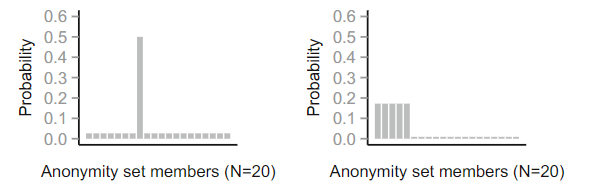
\includegraphics[scale=0.8]{pics/plot.png}
    \caption{Deux distributions\cite{anon_quantify}[9] avec la même cardinalité ($\approx$ 4.32 bits), 
    la même entropie de Shannon ($\approx$ 3.12 bits) et la même entropie normalisée 
    ($\approx$ 0.72)}
\end{figure}

La distribution de gauche a un émetteur avec une probabilité de $\frac{1}{2}$
et les 19 autres avec une probabilité de $\frac{1}{38}$.
La distribution de droite a 5 émetteurs avec une probabilité de $\frac{a}{5}$
et les 15 autres avec une probabilité de $\frac{1-a}{15}$ où $a \approx 0.86$
est la solution de l'équation définie par Toth dans \og Measuring anonymity\
revisited\fg. Un observateur capable d'enquêter uniquement un seul émetteur a une 
chance de réussite de 50\% dans la distribution de gauche et de 17.2\%
dans celle de droite. D'où l'utilisation de la min-entropie, une mesure 
conservatrice qui décrit l'imprévisibilité d'un résultat déterminé par la 
probabilité du résultat le plus probable. Cela correspond à la sécurité effective
dans le cas d'un observateur capable d'enquêter sur un seul émetteur. 
La min-entropie de la distribution de gauche est de 1 bit et celle de droite de 
$\approx$ 2.54 bits. Du point de vue du concepteur d'un système, on privilègera 
donc la distribution de droite à celle de gauche.

\begin{definition}[Min-entropie]
    $H_{min}(S) = - log_2(max \: p_i)$
\end{definition}



\section{Tableau de niveau de protection}
\begin{table}[!ht]
    \centering
    \begin{tabular}{|l|l|l|l|}
    \hline
        ~ & Bitcoin & Monero & Comment? (Monero) \\ \hline
        Anonymat de l'émetteur & Non & Oui (1/16) & Signature en anneau \\ \hline
        Anonymat du récepteur & Non & Oui & Adresse jetable \\ \hline
        Confidentialité des montants & Non & Oui & \acrshort{ringct} \\ \hline
        Révélation adresse \acrshort{ip} & ? & Non & Dandelion ++ \\ \hline
        Résistance au \acrshort{tga} & Non & Oui & Signature en anneau, adresse jetable, \acrshort{ringct} \\ \hline
    \end{tabular}
\end{table}

\clearpage 
\printglossaries 

\clearpage
\printbibliography

\end{document}